\documentclass[25pt, a0paper,
               colspace=15mm, subcolspace=0mm,
               blockverticalspace=17mm,
               landscape]{tikzposter} % See Section 

\usepackage{poster}
\usepackage{array}
\usepackage{multirow}
\usepackage{multicol}


\definecolor{PaleBlue}{rgb}{0,.55,.9}
\definecolor{PaleGreen}{rgb}{0,.7,.25}
\definecolor{RedPink}{rgb}{.9,0,.2}
\definecolor{Pink}{rgb}{.85,.35,.7}
\definecolor{Purple}{rgb}{.6,0,.75}
\definecolor{Orange}{rgb}{.9,.3,.05}

\colorlet{attentionColor}{Orange}
\colorlet{charEmbedColor}{RedPink}
\colorlet{predEmbedColor}{Pink}
% \colorlet{attentionColor}{GoldUL!90!black}
% \definecolor{attentionColor}{rgb}{.85,.5,.6}



\def\pathwidth{2pt}
\def\nodewidth{3pt}
\def\cornerCurvature{7pt}

\tikzstyle{embed}=[%
  draw,
  #1,
  % line width=3pt,
  anchor=north,
  minimum width=.8cm,
  minimum height=1.6cm,
  inner sep=0pt,
  text=#1!65!black,
  font=\fontsize{25pt}{24}\selectfont,
  ]

\title{\parbox{\linewidth}{\centering Pruning Filters In Convolution Neural Network}}
\institute{Department of Computer Science and Software Engineering, Université Laval}
\author{Vincent Martineau}

\begin{document}
\maketitle

\begin{columns}
\column{.4}
\block{Introduction}{%
We explore how reducing network expressivity can affect performance in Convolution Neural Network (CNN). We implemented a pruner that can remove filters from convolution layer and explore the effect on transfer learning tasks. 

\vspace{5mm}
\textbf{Motivations:}
\begin{itemize}
  \item \colorbold{Reduce} network size.
  % \item Goldberg (2017) emphasizes this fact for NLP tasks such as part of speech tagging (POS) or named entity recognition (NER).
  \item \colorbold{Improve} execution speed.
\end{itemize}

\vspace{5mm}
\textbf{Related work:}
\begin{itemize}
  \item P.Molchanov et al. (2017): Pruning Convolutional Neural Networks for Resource Efficient Inference.
\end{itemize}

\vspace{0mm}
\textbf{Goals:}
\begin{itemize}
  \item Evaluate the impact of reducing network expression on performance.
  \item Compare training time on various model.
  \item Compare various strategies to prune.
  \item Provide a module that could.
\end{itemize}
}

\column{0.30}
\block{Comparing Various Level of Pruning}{

\vspace{-15pt}

\begin{center}
	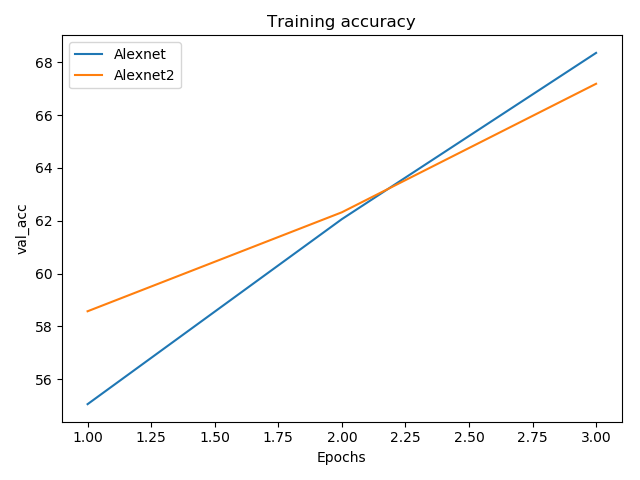
\includegraphics[width=25cm, height=15cm]{figures/prune_ratio}
\end{center}

This graph compare various level of pruning. Each level of pruning is made on two iteration made after 10 epochs of training and 3 epochs or retraining. Pretrained weight were used to see the impact on transfer learning.
}

\column{0.30}
\block{Comparing Pruning on  Multiple Models}{
	
	\vspace{-15pt}
	
\begin{center}
	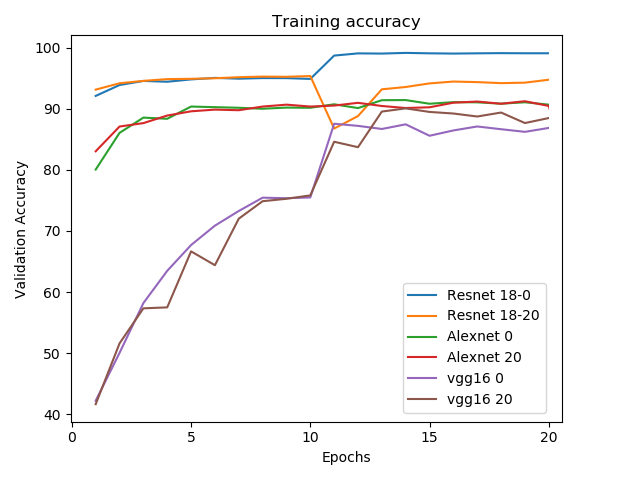
\includegraphics[width=25cm, height=15cm]{figures/various_models}
\end{center}

This graph explore the effect of pruning on different models. Each model shows the effect of pruning 20\% of the convolution filters in one step after 10 epochs of training. In this case transfer learning is not applied.
}
\end{columns}

\begin{columns}
\column{0.50}
\block{Example of Network Reduction}{
	
\vspace{-15pt}
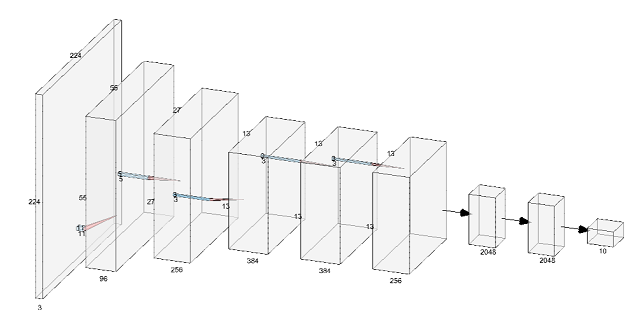
\includegraphics{figures/Alexnet_origin}
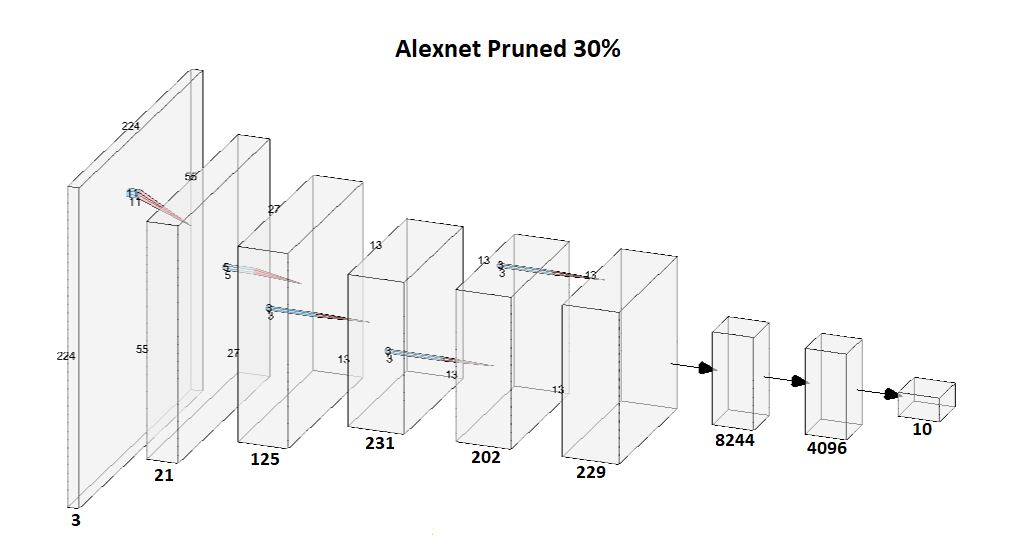
\includegraphics{figures/Alexnet_30}
	
	Comparing the effect of pruning on AlexNet. Left is the original model provided by pytorch. On the right is alex net pruned 30\%. In the case of network like Alexnet there is an important reduction of parameters based on the reduction of the fully connected layer. Their is also an important reduction in the first layers.
}


  \column{.25}
  \block{Algorithm}{
  	\begin{itemize}
  	\item Pretrain network with full paramters
  	\item Prepare pruning
  	\begin{itemize}
  	\item Convert model to ONNX
  	\item Extract execution graph
  	\item Determine which layer can be pruned
    \end{itemize}
  	\item Prune network
  	\item Reset optimizer
  	\item Finalize training
  \end{itemize}
 \vspace{45mm}
  }

  \column{.25}
\block{Settings}{
}

\end{columns}


\begin{columns}

  \column{.3}


  \block{Labeling task net}{

 
  % \vspace{3mm}

  Two nets working together: the first predicts OOV embeddings (see OOV handling net section) and the second one predicts tags.

  The simple architecture of the labeling net is used to emphasize the usefulness of our module, and to minimize the influence of other factors.

  \vspace{-.5mm}

  }









  \column{.3}
  \block{Observation}
  {
  	\begin{itemize}
   \item Not all convolutional layer can be pruned. Pruning layer before a residual connection is dangerous because both side of the residual connection must have the same side.
  \item When pruning in a convolution layer it is important to propagate. So the next layer have the right input size. This apply to convolution, linear and batchnorm layers.
  \item The algorithm used tend prefer removing filters that are deeper in the model and it is not uncommon to try to prune all filter in a layer.
  \item When pruning it is important to reset optimizer.
  \end{itemize}
  }







  
  
  
  \column{.4}
  

  \block{Performance gain}{%
  \begin{center}
  \setlength{\tabcolsep}{5mm}
  \begin{tabular}{c c c c c}
  \toprule
  \textbf{Task} & \textbf{Metric} & \textbf{Random Emb.} & \textbf{Our module} & \textbf{Gain}\\
  \midrule
  NER      & F1   & 77.56 & \colorbold{80.62} & 3.9\% \\
  POS      & acc. & 91.41 & \colorbold{92.58} & 1.2\% \\
  % Chunking & acc. & 92.63 & 93.16  & \textbf{93.19} \\
  % Keyphrase& F1   & 37.40 & 39.56 & \textbf{39.77} \\
  \bottomrule
  \end{tabular}
  \end{center}
  
  \vspace{2.5mm}
  The impact of our model on two NLP downstream tasks. We compare our OOV embeddings prediction scheme against random embeddings.
  \vspace{-12mm}
  }


  
  
  
  
  
  
  
  
  
  
  
  
  \block{Conclusion}{
  
  \textbf{Discussion:}
    \begin{itemize}
        \item \colorbold{Morphology} and \colorbold{context} help predict useful embeddings.
        \item \colorbold{The attention mechanism works}: depending on the task, the network will use either more the context or the morphology to generate an embedding.
    \end{itemize}
    
    \textbf{Future works:}
    \begin{itemize}
        \item  Apply the \colorbold{attention mechanism on each character of the OOV word and each word of the context} instead of using the hidden state of the respective elements only.
        \item Test our attention model in \colorbold{different languages} and on other NLP tasks, such as \colorbold{machine translation}.
    \end{itemize}
    \vspace{-3.5mm}
  }
\end{columns}

\end{document}
